\documentclass[conference,9pt,letterpaper]{IEEEtran}
\usepackage[T1]{fontenc}
\usepackage{newtxtext,newtxmath}
\usepackage{microtype}
\clubpenalty=10000
\widowpenalty=10000
\displaywidowpenalty=10000
\brokenpenalty=1000
\usepackage{graphicx}
\usepackage{booktabs}
\usepackage{amsmath}
\usepackage{array}
\usepackage{xcolor}
\usepackage{soul}
\DeclareRobustCommand{\pending}[1]{{\sethlcolor{yellow}\hl{#1}}}
\setlength{\abovecaptionskip}{3pt}
\setlength{\belowcaptionskip}{2pt}
\setlength{\intextsep}{6pt plus 1pt minus 1pt}
\setlength{\textfloatsep}{7pt plus 1pt minus 1pt}
\setlength{\floatsep}{6pt plus 1pt minus 1pt}
\usepackage{cite}
\usepackage{url}
\usepackage{stfloats}
\usepackage{balance}
\makeatletter
\patchcmd{\@BAlancecol}
 {\setbox\@leftcolumn=\vbox to \@tempdima}
 {\@tempdimb=\ht1\advance\@tempdimb by\dp1
  \ifdim\@tempdimb>\@tempdima\@tempdima=\@tempdimb\fi
  \@tempdimb=\ht3\advance\@tempdimb by\dp3
  \ifdim\@tempdimb>\@tempdima\@tempdima=\@tempdimb\fi
  \setbox\@leftcolumn=\vbox to \@tempdima}
 {\typeout{MECC: balance packing includes split-box depth.}}
 {\errmessage{Failed to patch balanced-column packing}}
% Stretch section and figure spacing instead of leaving unequal column tails.
\patchcmd{\@BAlancecol}{\unvbox1\vfil}{\unvbox1}
 {\typeout{MECC: balanced left column uses body glue.}}
 {\errmessage{Failed to patch left balance tail}}
\patchcmd{\@BAlancecol}{\vfil}{}
 {\typeout{MECC: balanced right column uses body glue.}}
 {\errmessage{Failed to patch right balance tail}}
\makeatother
\usepackage{capt-of}
\usepackage{float}
\usepackage{needspace}
\setcounter{dbltopnumber}{3}
\renewcommand{\dbltopfraction}{0.85}
\renewcommand{\textfraction}{0.10}
\newcommand{\mecc}{\textsc{MECC}}
\newcommand{\BH}{B_{\mathrm H}}
\newcommand{\BC}{B_{\mathrm C}}
\newcommand{\KH}{K_{\mathrm H}}
\newcommand{\KC}{K_{\mathrm C}}
\newtheorem{proposition}{Proposition}
\title{MECC: Single-GPU MoE Inference with\protect\\Compiler-Guided Three-Tier Expert Caching}
% Anonymous review copy: no author names or affiliation spacer rows.
\author{}
\usepackage[hidelinks]{hyperref}
\hypersetup{pdftitle={MECC: Single-GPU MoE Inference with Compiler-Guided Three-Tier Expert Caching},pdfauthor={}}
\begin{document}
\maketitle\flushbottom
\begin{abstract}
Expert offloading enables single-GPU inference for mixture-of-experts (MoE) models. Repeated HDD reads make expert residency a source of inference latency. We present MECC, the MoE Expert Cache Compiler, for profile-guided placement and joint HBM/CPU caching. Its compiler allocates slots by layer and emits the expert IDs used for initialization. The runtime promotes router-selected experts and retains displaced GPU weights in the host cache. The delivery path orders HDD reads and H2D copies before GPU consumption. On one A100, MECC gives 1.77$\times$ decode speedup over streaming on FP16 Mixtral-8x7B. First-token speedup reaches 2.86$\times$ over a Fiddler-style adapter. The evaluated Mixtral perplexity is 3.427. Joint retention reduces HDD demand by 73.9\% relative to independent caches.
\end{abstract}

\begin{IEEEkeywords}
Mixture of experts, single-GPU inference, expert offloading, three-tier caching, hardware/software co-design.
\end{IEEEkeywords}

\section{Introduction}
Mixture-of-experts (MoE) models scale parameter capacity through sparse expert activation~\cite{shazeer,switch,mixtral,deepseekmoe}. For example, Mixtral selects two of eight experts in each layer. A single-GPU deployment can use high-bandwidth memory (HBM), host memory, and a hard disk drive (HDD) to hold that pool. The selected expert's location determines its delivery path. HBM residents are ready for GPU execution; host residents require a host-to-device (H2D) copy; cold experts require an HDD read followed by H2D. Layer dependencies expose these reads on the inference critical path. Prefill can reuse fetched weights across prompt rows, and decoding can reuse them across output tokens. On shared servers, a serving task manages its expert allocation alongside other jobs and model instances. We study how to distribute that allocation across layers and retain weights for recurring requests. All MoE layers share the HBM and host allowances. Increasing one layer's allocation leaves fewer slots for others. The value of another slot depends on the demand already covered in that layer. Placement therefore couples the layers' local request distributions to a shared storage allocation.



Expert parallelism places experts across GPUs~\cite{deepspeedmoe,tutel,flashmoedist}. Single-GPU systems combine expert paging and caching~\cite{offloading,swapmoe,moeinfinity,promoe} with CPU/GPU execution~\cite{fiddler,daop,lightning}. MoE-CORE combines layer-wise allocation, profile initialization, and online replacement with cross-layer prefetching~\cite{core}. It also supports substitution for eligible expert misses. SSD-LLaMA retains GPU victims in RAM and pipelines storage delivery alongside lossless compression and CPU/GPU work partitioning~\cite{ssdllama}. Edge FlashMoE studies cache replacement for storage-backed expert access~\cite{flashmoe}. Within such a hierarchy, initial placement and later admission affect different requests. A profile determines which weights are available when serving begins. GPU turnover then determines which of those weights survive on the host. Promoting a CPU expert vacates a host position just as an HBM victim loses its GPU position. Using that position for the victim preserves its place in the reuse order. Figure~\ref{fig:intro} compares this joint rule with independent HBM/CPU caches on an A100. Joint retention gives 4.46$\times$ decode speedup over independent replacement and reduces HDD demand by 73.9\%. MECC also gives 1.77$\times$ speedup over streaming. These comparisons motivate retaining reusable expert weights across both memory tiers throughout serving.



\begin{figure}[!t]
\centering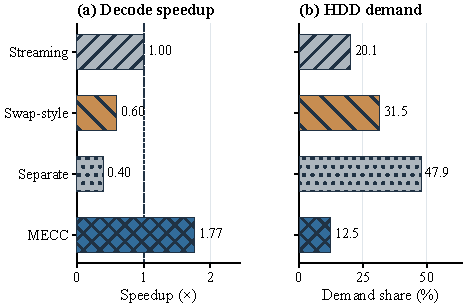
\includegraphics[width=\columnwidth]{measured_figures/intro_evidence.pdf}
\par\nointerlineskip
\caption{Mixtral-8x7B on one A100. Decode speedup is relative to streaming; Separate uses independent HBM/CPU caches. Swap-style is the SwapMoE-style adapter. Higher speedup and lower HDD demand are better.}
\label{fig:intro}
\end{figure}

We present \mecc{}, the MoE Expert Cache Compiler, to connect these two stages. Compilation ranks experts within each layer and allocates slots by marginal covered demand. The resulting plan specifies both per-layer capacities and the IDs loaded into HBM and CPU. The runtime maintains a joint recency order across those tiers. A CPU hit promotes the selected expert and demotes the GPU victim; a cold admission can also evict a host resident. A host mirror supplies the weights of each demoted GPU resident. Host admission reuses this copy through a metadata update. Stream tracking keeps tensor storage live through kernel execution. Runtime requests update membership within the compiled capacities. Weight delivery follows the selected experts' read and copy dependencies before GPU execution. Prefill submits cold reads for the active expert batch, while decode loads selected experts on demand. The compiler and runtime address each weight block by its layer/expert ID. This key connects a profiled rank to its initial location, later cache updates, and FP16 execution.

This paper makes three contributions.
\begin{list}{}{\setlength{\leftmargin}{16pt}\setlength{\labelwidth}{14pt}\setlength{\labelsep}{2pt}\setlength{\itemsep}{3pt}\setlength{\topsep}{3pt}}
\item[(1)] \textbf{Compiling initial residency.} We map layer profiles and expert allowances to per-layer capacities and ranked expert IDs. A marginal-coverage scan determines how each additional slot extends the initial resident set.
\item[(2)] \textbf{Updating cross-tier residency.} We connect the compiled state to joint promotion and victim demotion. Host retention preserves GPU evictions for later reuse, while read/copy ordering prepares selected weights for consumption.
\item[(3)] \textbf{Evaluating weight delivery.} We compare placement, retention, and scheduling through decode latency, first-token time, source-tier demand, and sample perplexity. Workload and capacity sweeps examine calibration, task transfer, prompt length, batch size, and host allocation. Deployment comparisons report latency and accelerator occupancy.
\end{list}
\twocolumn[{
\begin{minipage}{\textwidth}
\centering
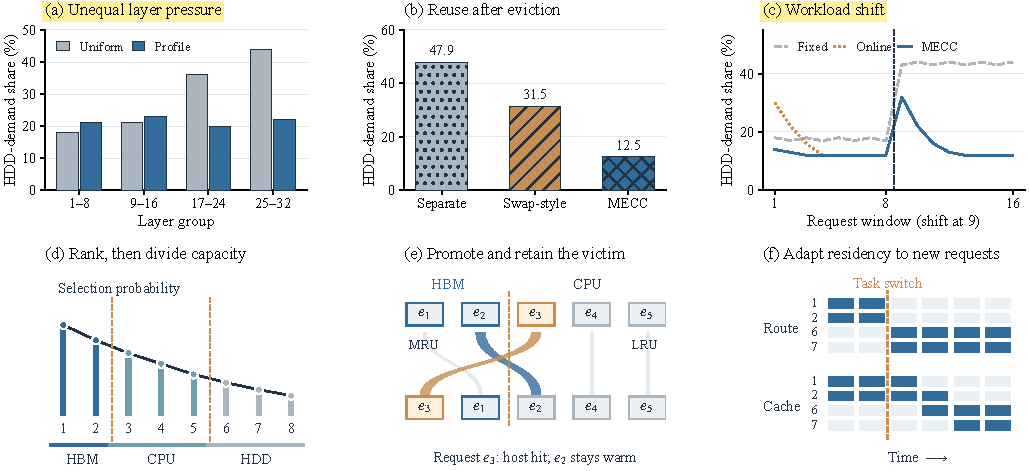
\includegraphics[width=\textwidth]{figures/fig02_motivation_insights.pdf}
\par\nointerlineskip
\captionof{figure}{Expert-cache behavior and MECC's three design choices. (a--c) compare layer pressure, cross-tier reuse, and workload change; (b) counts A100 demand across all phases. (d--f) show layer-specific capacity cuts, joint victim retention, and online membership updates.}
\label{fig:insights}
\vspace{5pt}
\end{minipage}
}]
\balance
\section{Background}
\label{sec:background}
\subsection{Sparse Execution, Full Weight Capacity}
An MoE layer routes each token to a subset of experts and combines their outputs~\cite{shazeer,switch,gshard}. Mixtral and the DeepSeek family separate active computation from the size of the stored expert pool~\cite{mixtral,deepseekmoe,deepseekv2,deepseekv3,mixtral22}. An expert belongs to one layer; equal indices at different layers identify different weights. For input $x$, let $G(x)$ be the selected set and $g_e(x)$ its normalized gate weights. The layer computes
\begin{equation}
y(x)=\sum_{e\in G(x)}g_e(x)E_e(x).
\end{equation}
Each gate produces expert requests as a token traverses the model. Decode revisits the layers for each output token. An expert request triggers a residency lookup, weight delivery, and execution on its assigned token rows. The gate weights then combine the expert outputs.

\subsection{Expert Residency on One GPU}
Expert parallelism places experts on GPU owners and dispatches token activations to them~\cite{deepspeedmoe,tutel,megablocks,flashmoedist,harmoeny}. Single-GPU offloading delivers selected weights to the execution device. Experts share HBM with dense weights, activations, and the KV cache~\cite{pagedattention,sglang}. The host cache supplies H2D copies; HDD supplies weights absent from both resident tiers. Heterogeneous inference systems combine these paths with CPU/GPU scheduling~\cite{flexgen,dsinference,zeroinfinity,llmflash,powerinfer,hetegen}. In prefill, several prompt rows can share a fetched expert. Decode advances one token per sequence, exposing fewer rows to each active expert. The amount of ready computation therefore changes between the two phases. Other systems change transfer size through precision selection~\cite{hobbit,specter}, expert segmentation~\cite{moepic,slicemoe}, or staging and compression~\cite{mira,zipmoe}.

Calibration counts determine expert ranking; runtime accesses determine recency. Within one layer, sequences $[a,a,b,b]$ and $[b,b,a,a]$ have equal counts and different last-access orders. MECC initializes from the ranked profile and replaces residents by recency.

\section{Motivation and Insights}
\label{sec:challenges}
\subsection{Allocating Slots by Marginal Demand}
Expert demand varies across layers. Some layers concentrate requests in a few ranks; others spread requests across more experts. Figure~\ref{fig:insights}(a,d) illustrates the resulting allocation choice. Its profile-guided plan shifts slots toward the layer groups with more cold demand. The compiler makes this choice by comparing each layer's next uncovered rank. Allocating a slot exposes that layer's following rank as a new candidate. This process distributes a shared allowance across layers and retains the IDs that fill each allocation. Routing locality across models has also been studied independently~\cite{routingconsistency}.

\subsection{Preserving Reuse after GPU Eviction}
A GPU victim is also a candidate for host admission. Figure~\ref{fig:insights}(b,e) shows a CPU promotion vacating a host position as the GPU selects its victim. Joint retention admits that victim into the vacated position, carrying recency across the tier boundary. Starting from the same allocation and expert order, joint retention reduces HDD demand from 47.9\% to 12.5\%. A demoted expert enters CPU MRU and remains available until subsequent admissions evict it from CPU LRU. A later selection promotes this host copy through H2D, turning the earlier GPU eviction into a host-cache hit.

\subsection{Updating Residency beyond Calibration}
Calibration and serving inputs can select different expert sets. In Figure~\ref{fig:insights}(c,f), a task switch moves requests toward a new expert set. MECC initializes the resident set from calibration and then admits experts requested during serving. Each admission updates recency and brings the cache closer to the active task. Repeated requests keep the new experts near MRU; their unused predecessors advance toward eviction. The profile supplies an initial hot set, and request-driven replacement tracks its evolution. The compiled capacities assign each layer the space used for this adaptation.

\twocolumn[{
\begin{minipage}{\textwidth}
\centering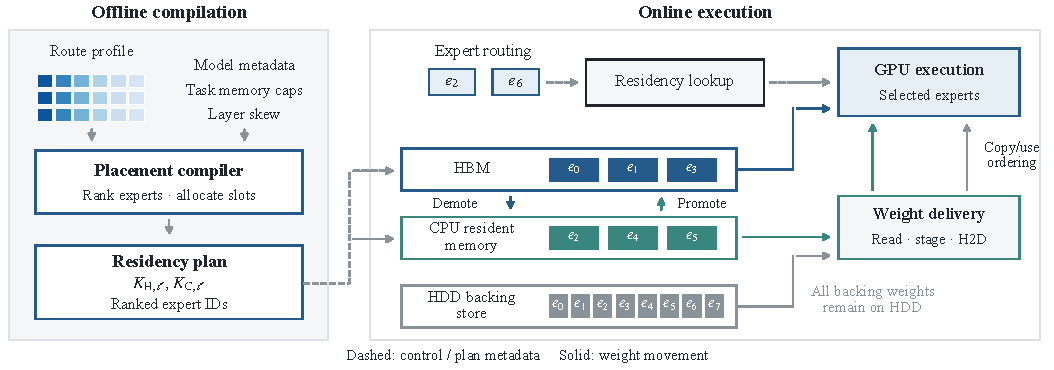
\includegraphics[width=\textwidth]{figures/fig01_overview.pdf}
\par\nointerlineskip
\captionof{figure}{MECC framework. The placement compiler emits per-layer capacities and ranked IDs. Online execution maps routed expert requests to HBM, CPU resident memory, or HDD, then supplies their weights to GPU computation. Dashed arrows carry control or plan metadata; solid arrows move weights.}
\label{fig:overview}

\vspace{8pt}
\end{minipage}
}]

\nobalance
\section{Overview}
\label{sec:overview}
Figure~\ref{fig:overview} follows the plan from profiling to GPU execution. The compiler receives layer/expert counts, skew parameters, model metadata, and expert allowances. It emits capacities and ranked IDs for each layer. Initialization loads the corresponding HBM and CPU residents; the complete expert pool remains on HDD. The runtime subsequently consumes this plan as an initial cache state.

Consider the selected experts $e_2$ and $e_6$ in the framework. The residency lookup finds $e_2$ on the host and $e_6$ in the backing store. Promoting $e_2$ frees a host position for an HBM victim. Loading $e_6$ then admits another GPU resident and updates the same tier order. The delivery path resolves each weight's read and copy before its consumer executes. The model combines the expert outputs using the gate weights and continues to the next layer.

Residency persists across tokens. Each layer updates its own membership within the compiled capacities. Per-layer recency carries request history from one token to the next. Promotions refresh the active experts, and demotions extend their reuse through host residency. Section~\ref{sec:method} specifies these transitions; Section~\ref{sec:evaluation} examines the resulting delivery cost.

\section{Method}
\label{sec:method}
\subsection{Compiling Capacities and Initial Identities}
\begin{figure}[H]
\centering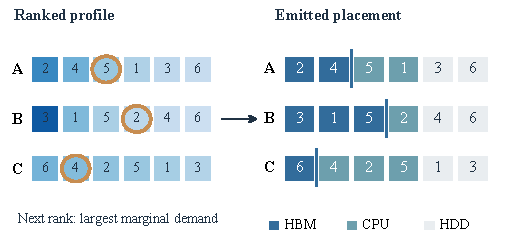
\includegraphics[width=\columnwidth]{method_redesign/compile_frontiers.pdf}
\par\nointerlineskip
\caption{Compiling the initial state. The left grid contains ranked per-layer demand; circles mark the next uncovered candidates. Shared HBM/CPU slot allowances produce different cuts in the emitted rows. A, B, and C identify different layers. }
\label{fig:compile}
\end{figure}

Consider $L$ MoE layers with $N_\ell$ experts per layer. Within each model, experts have equal size $s$ and layers use the same top-$k$.

Expert allowances $B_{\mathrm H}$ and $B_{\mathrm C}$ provide $S_{\mathrm H}=\lfloor B_{\mathrm H}/s\rfloor$ HBM slots and $S_{\mathrm C}=\lfloor B_{\mathrm C}/s\rfloor$ CPU slots.

For each layer, the compiler receives an expert order and a skew parameter $\alpha_\ell$. Profile counts determine the order. A discrete Zipf model gives the probability associated with each rank:
\begin{equation}
q_{\ell,r}=\frac{r^{-\alpha_\ell}}{\sum_{j=1}^{N_\ell}j^{-\alpha_\ell}},
\qquad p_{\ell,r}=q_{\ell,r}/L.
\end{equation}
Here $q_{\ell,r}$ is conditional on an access to layer $\ell$. Equal top-$k$ gives equal selection mass across layers. Each rank stores the layer-local ID of its expert weight block.

Figure~\ref{fig:compile} shows the HBM and CPU cuts in those lists. Capacities satisfy $\sum_\ell K_{\mathrm H,\ell}\le S_{\mathrm H}$, $\sum_\ell K_{\mathrm C,\ell}\le S_{\mathrm C}$, and $K_{\mathrm H,\ell}+K_{\mathrm C,\ell}\le N_\ell$. The adaptive scan reserves one slot per layer in each fast tier, then distributes the remaining slots by marginal coverage.

The scan first assigns HBM slots. At each step, it chooses the layer with the largest next-rank score:
\begin{equation}
\Delta_\ell=q_{\ell,K_{\mathrm H,\ell}+1}.
\end{equation}
CPU allocation continues from the first ranks beyond each HBM cut. Every allocation exposes a new next-rank candidate in that layer. Layer ID breaks score ties, and expert ID breaks count ties. The direct scan takes $O(L(S_{\mathrm H}+S_{\mathrm C}))$ time after sorting. Its score is the request probability covered by the next slot.

The emitted plan contains the final capacities and ordered expert IDs. Initialization places each layer's first HBM ranks on the GPU and its next CPU ranks on the host. Natural ID order initializes the uniform control. During execution, admission changes membership within the compiled capacities.

\subsection{Retaining Victims across the Tier Boundary}
Each layer maintains two ordered sets, from most-recently used (MRU) to least-recently used (LRU). Their concatenation places HBM residents before CPU residents. An HBM hit moves its expert to HBM MRU. A CPU hit removes its host entry and promotes it to HBM MRU. The GPU LRU victim then becomes CPU MRU. A cold admission follows the same GPU insertion and can remove the CPU LRU. HDD retains the backing weights for every expert.

\begin{figure}[H]
\centering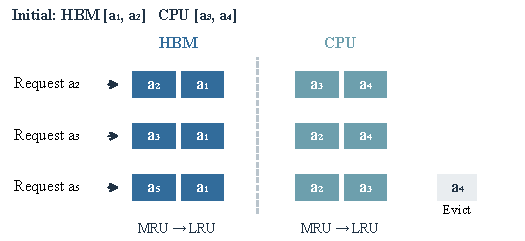
\includegraphics[width=\columnwidth]{method_redesign/residency_cases.pdf}
\par\nointerlineskip
\caption{Residency transitions for three requests. An HBM hit refreshes recency; a CPU hit promotes the requested expert and demotes a GPU victim; cold admission also removes a CPU victim. Rows give the resulting MRU-to-LRU order.}
\label{fig:retention}
\end{figure}
Each row in Figure~\ref{fig:retention} starts from HBM $[a_1,a_2]$ and CPU $[a_3,a_4]$. An $a_2$ hit changes the GPU order. Promoting $a_3$ releases its CPU position, which receives the HBM victim $a_2$. A cold $a_5$ request first enters HBM and pushes its GPU victim into the full host cache. The host LRU $a_4$ then leaves the resident set. Promotion recycles the requested expert's CPU position; cold admission obtains a position through host eviction.

The resulting order extends from HBM MRU through CPU LRU. Requests enter at its front, and capacity pressure removes experts at its tail. During batch preparation, the loader can prepare several active experts. Temporary references hold their weights until each expert processes its token rows.

Each GPU resident carries a host mirror. Demotion admits this mirror to the CPU cache through a metadata update, saving a device-to-host copy. Tracking the consumer stream keeps tensor storage live until kernel execution completes.

\subsection{Ordering Delivery before Expert Consumption}
Prefill groups token rows by selected expert and submits the corresponding cold reads. Each read is resolved when its expert reaches consumption. Figure~\ref{fig:delivery} shows resident work overlapping a pending read for another selected expert. Decode delivers each requested expert on demand. The expert kernel processes its assigned rows, and the gate weights combine the resulting outputs.

\begin{figure}[H]
\centering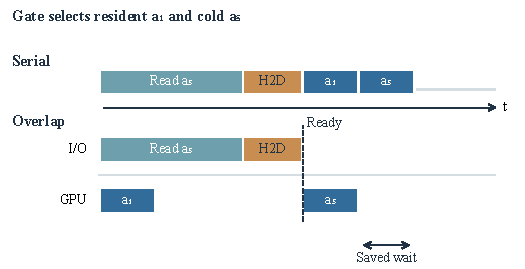
\includegraphics[width=\columnwidth]{method_redesign/delivery_overlap.pdf}
\par\nointerlineskip
\caption{Prefill delivery for resident $a_1$ and cold $a_5$. Computing $a_1$ overlaps the pending read for $a_5$. H2D completion releases $a_5$ for GPU execution; the shortened schedule saves exposed waiting time. }
\label{fig:delivery}
\end{figure}
A read future returns the host tensors that supply H2D. The copy stream moves them to the GPU and synchronizes before the loader yields the device tensors. The expert kernel then consumes those tensors. Recording its stream extends their lifetime through kernel completion. This read--copy--compute chain connects storage delivery to the expert's execution point.

Prefetchers use profiles or lookahead to anticipate expert demand~\cite{pregated,fate,expertflow}. Batch and request schedulers expose work from concurrent inputs~\cite{klotski,bevy}; distributed edge schemes add network delivery~\cite{odmoe}. MECC schedules the expert work already selected at the current gate. Retention removes repeated reads and copies. Overlap shortens the exposed part of the remaining delivery.

\subsection{Resolving Requests to Expert Execution}
The execution interface accepts a layer/expert ID and its assigned token rows. Lookup resolves the ID to resident tensors or a backing-store block. Delivery prepares GPU weights for the expert projections. Gate weights combine their outputs before execution advances to the next layer.

\section{Evaluation}
\label{sec:evaluation}
\subsection{Evaluation Overview}
We evaluate decode and first-token speedup, source-tier demand, and workload sensitivity. Phase speedup divides the streaming latency by the policy latency. The main comparison includes SwapMoE-style retention and Fiddler-style CPU computation~\cite{swapmoe,fiddler}. Component studies examine allocation, victim retention, and delivery scheduling. Workload sweeps vary calibration, task transfer, input length, and batching. Appendix~\ref{app:setup} provides configuration details and the complete measured policy results.

\subsection{Single-GPU Performance}
\begin{figure}[H]
\centering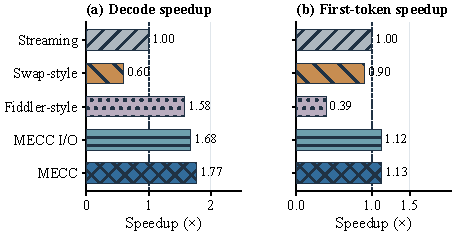
\includegraphics[width=\columnwidth]{measured_figures/main.pdf}
\par\nointerlineskip
\caption{Decode and first-token speedup on one A100, relative to streaming (1.0). Swap-style and Fiddler-style denote the corresponding mechanism adapters. MECC I/O varies the weight-delivery path. Higher is better.}
\label{fig:performance}
\end{figure}
Figure~\ref{fig:performance} reports 1.77$\times$ decode and 1.13$\times$ first-token speedup for MECC over streaming. Against Fiddler-style CPU computation, the gains are 1.12$\times$ and 2.86$\times$, respectively. GPU execution reuses each fetched expert across its selected prompt rows. This reuse has more work to cover during prefill, accounting for the different phase tradeoffs. Response length determines how these initial and recurring costs contribute to completion time.

MECC serves 77.5\% of classified expert accesses from HBM and 10.0\% from the host cache. The remaining 12.5\% reach HDD. Each host hit replaces a storage read with an H2D copy; each HBM hit directly supplies GPU computation. Promoting a host resident creates room for the displaced GPU expert, extending its retention into the next tier. Later requests can reuse this host copy after its GPU slot has been reassigned. The access distribution captures the resulting use of the three delivery paths.

Joint retention gives 2.95$\times$ decode speedup over the SwapMoE-style adapter. Against independent replacement, the gain is 4.46$\times$, accompanied by 73.9\% lower HDD demand in Figure~\ref{fig:intro}. These results link cross-tier retention to the cost of repeated weight delivery. Component studies next examine allocation, retention, and scheduling.

\begin{figure*}[!t]
\centering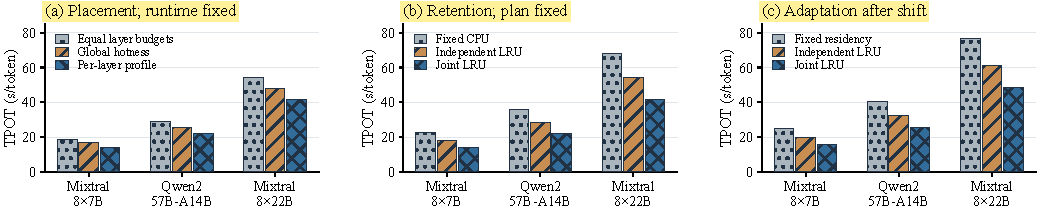
\includegraphics[width=\textwidth]{completion_figures/mechanism_sweeps.pdf}
\par\nointerlineskip
\caption{Component comparisons on three models. (a) Placement with runtime fixed. (b) Retention with initialization fixed. (c) Adaptation after a task switch. }
\label{fig:target_mechanisms}
\end{figure*}
\Needspace*{12\baselineskip}
\subsection{Mechanism Attribution}
\label{sec:mechanisms}

Figure~\ref{fig:target_mechanisms} varies one decision in each panel. The placement comparison keeps the runtime rule fixed; retention keeps initialization fixed; adaptation follows a task switch. For Mixtral-8x7B, per-layer placement changes TPOT from \pending{18.6 to 14.2 s/token}. Joint retention changes it from \pending{18.3 to 14.2}, and online adaptation changes the post-switch value from \pending{25.1 to 16.0}. The same comparisons span three models, relating each mechanism to its allocation or request sequence.

\begin{figure}[H]
\centering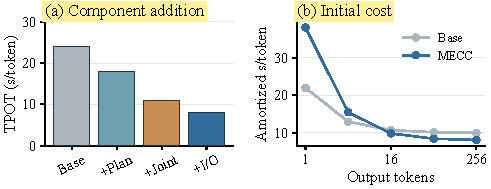
\includegraphics[width=\columnwidth]{completion_figures/ablation_startup.pdf}
\par\nointerlineskip
\caption{Ablation and startup. The right panel reports initialization cost per output token plus decode cost.}
\label{fig:target_ablation}
\end{figure}
Adding placement, joint retention, and I/O scheduling gives the TPOT sequence \pending{24, 18, 11, and 8 s/token} in Figure~\ref{fig:target_ablation}(a). The successive reductions are \pending{6, 7, and 3 s/token}. Joint retention provides the largest step by keeping GPU victims available on the host. Scheduling then shortens the delivery path at \pending{20 percent} HDD demand. Panel (b) includes the initial placement cost, connecting this decode gain to the response length.

\begin{figure}[H]
\centering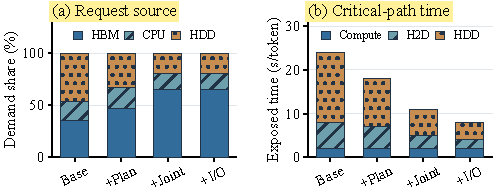
\includegraphics[width=\columnwidth]{completion_figures/traffic_exposure.pdf}
\par\nointerlineskip
\caption{Source demand and exposed time. The I/O step shortens exposed read/copy time at the final request-source distribution.}
\label{fig:target_traffic}
\end{figure}
Figure~\ref{fig:target_traffic} separates changes in demand from changes in exposed time. Placement and joint retention lower HDD demand from \pending{46 to 20 percent}. The final I/O configuration has an HBM/CPU/HDD mix of \pending{65/15/20 percent}. Its TPOT reduction from \pending{11 to 8 s/token} comprises \pending{2 seconds} less exposed HDD time and \pending{1 second} less exposed H2D time. The compute component remains at \pending{2 seconds}. Scheduling brings transfer completion closer to ready computation. Retention and overlap therefore act on two parts of delivery cost: the number of transfers and their exposed duration.

\subsection{Model and Deployment Scaling}
\begin{figure}[H]
\centering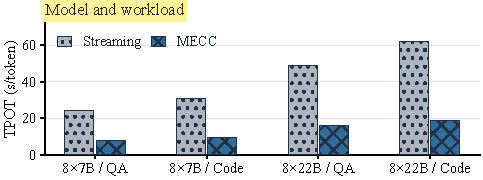
\includegraphics[width=\columnwidth]{completion_figures/cross_model.pdf}
\par\nointerlineskip
\caption{Model and workload comparison. Mixtral-8x7B and 8x22B with QA/code inputs. Each policy uses the same model and workload within a group. }
\label{fig:target_models}
\end{figure}
In Figure~\ref{fig:target_models}, MECC's speedup over streaming spans \pending{3.00--3.26}$\times$ across the four model/workload groups. The absolute TPOT difference grows from \pending{16 seconds} on 8x7B QA to \pending{43 seconds} on 8x22B Code. Moving from 8x7B to 8x22B \pending{doubles} MECC TPOT; the corresponding streaming increase is \pending{2.00--2.04}$\times$. The larger model therefore saves more delivery time per token at a comparable speedup.

\begin{figure}[H]
\centering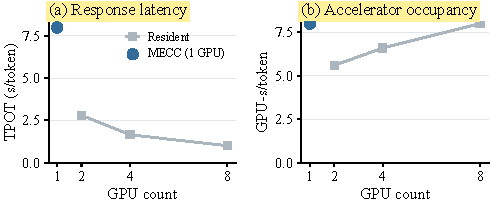
\includegraphics[width=\columnwidth]{completion_figures/gpu_tradeoff.pdf}
\par\nointerlineskip
\caption{One-GPU/resident-reference tradeoff. The panels compare single-GPU MECC with resident configurations and report latency alongside GPU occupancy.}
\label{fig:target_gpu}
\end{figure}
The endpoints in Figure~\ref{fig:target_gpu} pair \pending{one GPU at 8 s/token with eight GPUs at 1 s/token}. Both use \pending{8 GPU-s/token}, with different response times. The \pending{two-GPU resident point uses 5.6 GPU-s/token}. Plotting the intermediate configurations shows how accelerator provisioning changes both latency and occupancy. The single-GPU point quantifies the latency of supplying weights through the memory hierarchy.

\begin{figure*}[!t]
\centering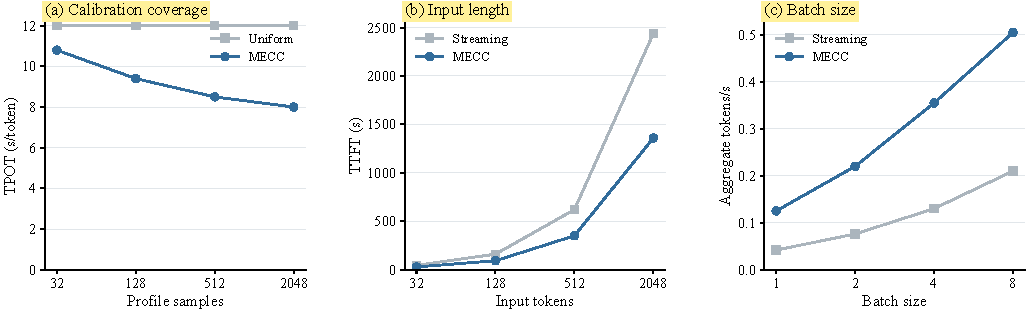
\includegraphics[width=\textwidth]{completion_figures/workload_sensitivity.pdf}
\par\nointerlineskip
\caption{Profile, input-length, and batch sensitivity. Profile size changes initialization quality, input length changes first-token work, and batch size changes aggregate throughput. The panels vary one workload parameter at a time.}
\label{fig:target_sensitivity}
\end{figure*}
\subsection{Capacity and Workload Sensitivity}

MECC gives 1.42$\times$ and 5.17$\times$ decode speedup over streaming at 30 and 60~GB. HDD demand falls from 32.2\% to zero as resident capacity covers all eight experts per layer.

\begin{figure}[H]
\centering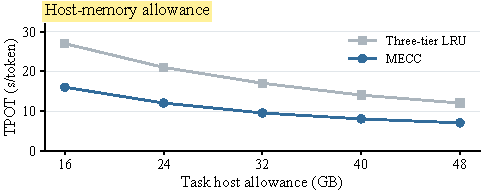
\includegraphics[width=\columnwidth]{completion_figures/quota_targets.pdf}
\par\nointerlineskip
\caption{Decode latency across host-memory allowances.}
\label{fig:target_quota}
\end{figure}
Figure~\ref{fig:target_quota} resolves the capacity range between sparse and broader host retention. MECC changes from \pending{16 to 7 s/token} across \pending{16--48 GB}; three-tier LRU changes from \pending{27 to 12}. The first host increment saves \pending{4 seconds/token} for MECC, while the final increment saves \pending{1 second/token}. Earlier slots can retain victims with shorter reuse distances. Additional slots then cover less frequent returns. This diminishing latency reduction complements the coverage transition at 60~GB, where the primary resident sets contain every expert.

\begin{figure}[H]
\centering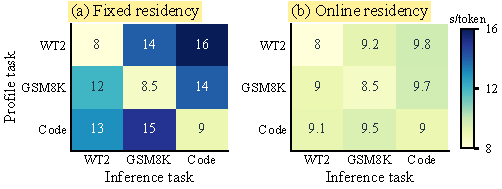
\includegraphics[width=\columnwidth]{completion_figures/profile_mismatch.pdf}
\par\nointerlineskip
\caption{Profile transfer across tasks. Rows select the calibration task and columns the inference task. Cells are TPOT in s/token; the two panels share a color scale.}
\label{fig:target_mismatch}
\end{figure}
Figure~\ref{fig:target_mismatch} separates within-task calibration from transfer to another task. The mean diagonal TPOT is \pending{8.50 s/token} under both fixed and online residency. Across the six off-diagonal pairs, the mean changes from \pending{14.00 to 9.38 s/token}, a \pending{33.0 percent} reduction. Request-driven admission brings the cross-task resident set toward the experts selected by the serving workload. The response to calibration size in Figure~\ref{fig:target_sensitivity}(a) addresses a different effect: how much profile information is available before the first request.

\balance
\subsection{Calibration Coverage and Input Length}
Increasing calibration from \pending{32 to 2048 samples} changes TPOT from \pending{10.8 to 8.0 s/token} in Figure~\ref{fig:target_sensitivity}(a). The final expansion yields a smaller reduction than the first. Once the ranked hot set stabilizes, additional samples affect fewer initial placements.

Figure~\ref{fig:target_sensitivity}(b) scales the prompt from \pending{32 to 2048 tokens}. MECC's TTFT changes from \pending{28 to 1360 seconds}, compared with \pending{45 to 2440} for streaming. Their endpoint speedups are \pending{1.61}$\times$ and \pending{1.79}$\times$. Prompt rows selected for the same expert can share one fetched weight block. Increasing input length thus exposes more opportunities to amortize delivery within prefill, alongside the increase in prompt computation.

\subsection{Batch Throughput and Sequence Progress}
Figure~\ref{fig:target_sensitivity}(c) reports aggregate output rate. Moving from \pending{one to eight sequences} increases MECC throughput from \pending{0.125 to 0.505 tokens/s}, or \pending{4.04}$\times$. The additional sequences share fetched expert weights and introduce more active rows at each gate.

For a synchronous batch of $B$ sequences with aggregate rate $R(B)$, the interval between batch steps is $B/R(B)$. The plotted MECC rates give \pending{8.00 seconds} at batch one and \pending{15.84 seconds} at batch eight. Batching therefore processes more tokens per unit time while increasing the interval between successive tokens of one sequence.

\subsection{Amortizing Initial Placement}
\label{sec:amortization}
Let $\Delta I$ denote the extra initialization time and $\Delta D$ the per-token decode saving. Equating the amortized per-token times gives the crossing $n^\star=\Delta I/\Delta D$. Figure~\ref{fig:target_ablation}(b) uses \pending{18 seconds} of extra initialization and \pending{2 seconds} of decode saving, yielding \pending{9 output tokens}. Longer responses recover the placement cost and retain part of the decode gain.

At \pending{64 output tokens}, initialization contributes \pending{0.47 s/token} for MECC and \pending{0.19} for the reference. Their total averages become \pending{8.47 and 10.19 s/token}, respectively. When requests share a resident cache, their output tokens amortize the same initialization. The cache lifetime determines the amortization horizon.

\section{Conclusion}
MECC combines profile-guided initial placement with joint HBM/CPU retention for single-GPU MoE inference. Its allocation and admission rules reduce repeated weight delivery, while scheduling overlaps the remaining read/copy work with ready expert computation. On one A100, MECC gives 1.77$\times$ decode speedup over streaming and 1.12$\times$ over the Fiddler-style adapter.

\clearpage
\balance
\bibliographystyle{IEEEtran}
\bibliography{references}
\clearpage
\appendices
\balance
\section{Experimental Configuration and Figure Data}
\label{app:setup}
\subsection{Hardware and Weight Representation}
The testbed uses one NVIDIA A100 80~GB PCIe with FP16 expert weights. Dense layers and the router execute on the GPU. The expert store is a RAID logical volume reporting ROTA=1, called HDD in this paper. The controller's physical-drive inventory remains unverified. Each expert block contains gate, up, and down tensors identified by layer and expert ID. HDD retains the complete expert pool.

\subsection{Measured Protocols}
The main comparison uses Mixtral-8x7B-Instruct-v0.1 with uniform initialization, four HBM slots and three CPU slots per layer. Planner allowances are 50/40~GB. Each policy runs once on eight WikiText-2 prompts with 64 input and 64 output tokens. PPL uses a 1024-token WikiText-2 sample. The loader and model graph are shared.

Raw TPOT in seconds is 13.04 for streaming, 21.75 for SwapMoE-style, 8.26 for Fiddler-style, 7.19 for FlashMoE-RF, 7.78 for MECC I/O, and 7.38 for MECC. Independent caching gives 32.94. TTFT is 156.86 seconds for streaming, 139.14 for MECC, 398.45 for Fiddler-style, and 101.76 for FlashMoE-RF. Plotted speedup divides the streaming phase latency by policy latency using unrounded JSON fields. The additional FlashMoE-RF adapter gives 1.81$\times$ decode and 1.54$\times$ first-token speedup over streaming. These complete policy results supplement the five-policy main figure.

The separate 30/60~GB host comparison uses four WikiText-2 prompts, 16 output tokens, and four HBM slots per layer. At 60~GB, four HBM and four CPU slots cover all eight experts per layer.

\subsection{Policy Definitions}
Streaming retains the initialized HBM set and fetches misses without GPU admission. The SwapMoE-style FP16 adapter uses a fixed CPU set and GPU LRU replacement. Fiddler-style computes non-HBM experts on the CPU. Both are local mechanism implementations. Independent caching updates HBM/CPU recency separately; MECC couples GPU promotion to victim demotion. MECC I/O is a separate delivery control.

FlashMoE-RF combines public inverse-recency and frequency features with equal weights, using HBM LRU. Its host score is $0.5/d_e+0.5f_e/f_{\max}$, with request distance $d_e$ and count $f_e$. The lowest score is evicted; ID breaks ties. The original trained predictor is absent. The main figure abbreviates SwapMoE-style as Swap-style. MoE-CORE and MoE-Infinity have no completed run in this repository.

\subsection{Timing and Demand Counters}
TTFT is time to first token; TPOT is time per output token during decode. Accelerator occupancy is GPU count times TPOT, in GPU-s/token. Measured HDD-demand shares aggregate classified accesses across instrumented phases. Prefetched experts are classified by residency at consumption. These shares are separate from physical read/copy byte counters and decode-only demand. The short-window diagnostic compares streaming and MECC routing, logits, gates, and tokens through their shared dispatch; it is not independent full-model equivalence evidence.

\subsection{Figure Data Annotations}
Yellow-highlighted values and panel titles identify authored design targets: unmeasured values specifying the illustrated comparisons. Introduction and main-runtime plots use committed A100 measurements. Motivation panel (b) uses measured aggregate demand; panels (a,c) use design arrays. Panels (d--f), the framework, and method figures are mechanism examples.

Component, startup, traffic/exposure, cross-model, GPU-occupancy, quota, sensitivity, and profile-transfer plots use design targets. Model names, QA/Code groups, and WikiText-2/GSM8K labels specify intended comparisons, not additional completed benchmark runs. Startup uses $T_{\mathrm{avg}}(n)=T_{\mathrm{init}}/n+T_{\mathrm{decode}}$. Demand stacks sum to 100\%; exposed-time stacks sum to component TPOT. Derived differences, speedups, off-diagonal means, and batch-step intervals use the same unmeasured arrays. They are arithmetic summaries, not additional runs.

\subsection{Memory and Execution Accounting}
Planner allowances count primary slots. GPU host mirrors and staging add physical host allocations; equal slot counts do not establish equal peak host bytes. The compiler library accepts per-layer skew and ranked IDs. The non-uniform e2e CLI generates skew; calibration is a separate compiler input. The measured main run uses uniform initialization. Prefill submits selected-batch read futures; decode uses demand delivery. Copy-stream synchronization orders CUDA consumption, and consuming-stream tracking preserves tensor lifetime.

\subsection{Source Records}
Committed run JSONs supply measurements. The measured-figure and ratio audits record run IDs, fields, raw latencies, and SHA-256 hashes. The two design-array files supply highlighted figures and retain their source hashes. Each archived manuscript includes its source and artifact hash record.

\end{document}
